% 美赛模板:正文部分

\documentclass[12pt]{article}  % 官方要求字号不小于 12 号,此处选择 12 号字体
% \linespread{1.1}
% \bibliographystyle{plain}
% 本模板不需要填写年份,以当前电脑时间自动生成
% 请在以下的方括号中填写队伍控制号
\usepackage[2107542]{easymcm}  % 载入 EasyMCM 模板文件
\problem{C}  % 请在此处填写题号
% \usepackage{mathptmx}  % 这是 Times 字体,中规中矩 
\usepackage{palatino}  % mathpazo 这palatino是 COMAP 官方杂志采用的更好看的 Palatino 字体,可替代以上的 mathptmx 宏包
\usepackage{pdfpages}
\usepackage{longtable}
\usepackage{tabu}
\usepackage{threeparttable}
\usepackage{listings}
\usepackage{paralist}
\usepackage{setspace}
\usepackage{appendix}


 \let\itemize\compactitem
 \let\enditemize\endcompactitem
% \let\enumerate\compactenum
% \let\endenumerate\endcompactenum
% \let\description\compactdesc
% \let\enddescription\endcompactdesc
% \usepackage{biblatex} 
% \usepackage{cite}
% \usepackage{natbib}
\newcommand{\upcite}[1]{\textsuperscript{\textsuperscript{\cite{#1}}}}
\title{A Glimpse of Machine Learning through Wordle}  % 标题

% 如需要修改题头(默认为 MCM/ICM),请使用以下命令(此处修改为 MCM)
%\renewcommand{\contest}{MCM}

% 文档开始
\begin{document}
\begin{abstract}
	In this paper, we analyze the game data posted on twitter by the \emph{New York Times} wordle game players, and provide a method to accomplish the task of analyzing the features of words and quantifying them, and predicting the number of participants and score distribution (The distribution of player attempts) reported on twitter on a future day based on the words of that day.

In this paper, we first present a method for predicting the number of participants based on the ARIMA model. We demonstrate a process that includes data pre-processing, smoothness testing, parameter selection, and error analysis, and apply the ARIMA model to the problem of predicting the number of reports on a future day based on previous data. A series of validations proved the excellent generalization ability of the model and the accuracy of the prediction described by MSE.

Then, we collected information on the daily usage frequency of words, word roots, and word properties as word features, completed the modeling of wordle words, and used the mean and standard deviation of the distribution of the number of player attempts as a measure of game difficulty. Four metrics describing the impact of words in the game (frequency of daily use, maximum number of repeated letters (MNRL), wordness, and number of word roots) were finally obtained. After ANOVA and calculation of Spearman's correlation coefficient, we found that MNRL significantly affects the percentage of player attempts in the difficult mode, and the larger the MNRL, the higher the percentage of players with multiple attempts and the lower the percentage of players with fewer attempts. The other three indicators do not correlate well with the percentage of attempts.

Next, we fitted the relationship between word and date and the number of player attempts using linear regression, and creatively regressed the percentage of players in seven categories using the parameters of the predicted probability distribution model instead. The problem that the results of linear regression are difficult to be constrained is solved by first predicting the probability distribution function and then calculating the percentage of 7 types of players by the probability distribution function. After analysis, we find that the discrete Gaussian distribution fits the proportion of players in 7 categories better, and the model built by this can achieve a small generalization error.

Then, based on the previous modeling of words and the quantification of difficulty, we also used the hierarchical clustering method to finish the grading of word difficulty, and finally chose the rule of two grades of hard and easy to be more reasonable. After that, we used the WSS formula to measure the impact of each word feature on difficulty MNRL>frequency of use>word nature>number of root words. Finally, an SVM-based word classifier was built to classify unfamiliar words in two grades of difficulty and ease.

In addition, we did many tests to ensure the generalization ability of the above model. And data exploration was done on the dataset to find some interesting properties about player features and player distribution. For example, we found that players in hard mode are harder to lose but also harder to grow; the mean and variance of player attempts also follow normal distribution well, etc.

% Translated with www.DeepL.com/Translator (free version)

	% \vspace{5pt}
	% \textbf{Keywords}: Markov chains, Random forest algorithm, Hierarchical clustering 
	
\end{abstract}
    
\maketitle  % 生成 Summary Sheet

\tableofcontents




% 正文开始
% Chapter 1: Introduction
\section{Introduction}

\subsection{Problem Background}
Music has been part of human societies since the beginning of time as an essential component of cultural heritage. There are many factors that can influence an artist's music making, especially between artists. The Integrative Collective Music (ICM) Society has asked our team to develop a model that measures musical influence, examining evolutionary and revolutionary trends of artists and genres.
The team are provided with the following tasks:

\begin{itemize}
	\setlength{\parsep}{0ex} %段落间距
	\setlength{\topsep}{2ex} %列表到上下文的垂直距离
	\setlength{\itemsep}{1ex} %条目间距
	\item We use the ARIMA model to predict the number of participants in the report at a future date, giving a prediction interval. A series of tests were conducted to ensure the generalization ability.
	\item We precisely collected and quantified the word frequency, MNRL (Maximum Number of Repeated Letters), root words, and word properties of the words in the dataset to model the wordle words.  
	\item We used the mean and standard deviation of the number of player attempts as the word difficulty. We divided the word features into two categories: discrete and continuous data, and evaluated the correlation between them and the mean and standard deviation of attempts, respectively. For the discrete data, we used ANOVA to assess the correlation between the different values. For continuous data, we assessed the correlation between the two continuous data by calculating the Spearman correlation coefficient.  
	\item We predicted the mean as well as the standard deviation of the number of player attempts based on the four indicators of the word and the date through a linear regression model, and ensured the effect by fitting the player distribution with a probability distribution model.
	\item For the classification problem, we used a hierarchical clustering method to file the difficulty of all words based on the previously modeled word features, and used the WSS formula to measure the contribution of the four indicators of word attributes to the results and find the word attributes that contribute the most to the results.
	\item A prediction model for classifying word difficulty based on word attributes was developed to analyze the word attributes of the word EERIE to determine the difficulty of the word. The model performance is analyzed by calculating the corresponding accuracy, recall, and other metrics of the model.  
	\item In addition, we deeply mined the dataset and found some interesting properties.
\end{itemize}

\subsection{Our work}

\begin{enumerate}[\bfseries 1.]
	\setlength{\parsep}{0ex} %段落间距
	\setlength{\topsep}{2ex} %列表到上下文的垂直距离
	\setlength{\itemsep}{1ex} %条目间距
	\item We use the ARIMA model to predict the number of participants in the report at a future date, giving a prediction interval. A series of tests were conducted to ensure the generalization ability.
	\item We precisely collected and quantified the word frequency, MNRL (Maximum Number of Repeated Letters), root words, and word properties of the words in the dataset to model the wordle words.  
	\item We used the mean and standard deviation of the number of player attempts as the word difficulty. We divided the word features into two categories: discrete and continuous data, and evaluated the correlation between them and the mean and standard deviation of attempts, respectively. For the discrete data, we used ANOVA to assess the correlation between the different values. For continuous data, we assessed the correlation between the two continuous data by calculating the Spearman correlation coefficient.  
	\item We predicted the mean as well as the standard deviation of the number of player attempts based on the four indicators of the word and the date through a linear regression model, and ensured the effect by fitting the player distribution with a probability distribution model.
	\item For the classification problem, we used a hierarchical clustering method to file the difficulty of all words based on the previously modeled word features, and used the WSS formula to measure the contribution of the four indicators of word attributes to the results and find the word attributes that contribute the most to the results.
	\item A prediction model for classifying word difficulty based on word attributes was developed to analyze the word attributes of the word EERIE to determine the difficulty of the word. The model performance is analyzed by calculating the corresponding accuracy, recall, and other metrics of the model.  
	\item In addition, we deeply mined the dataset and found some interesting properties.
\end{enumerate}


% \section{Introduction}
% \subsection{Problem Background}
% Here is the problem background ...

% Two major problems are discussed in this paper, which are:
% \begin{itemize}
%     \item Doing the first thing.
%     \item Doing the second thing.
% \end{itemize}

% \subsection{Literature Review}
% A literatrue\cite{1} say something about this problem ...

% \subsection{Our work}
% We do such things ...

% \begin{enumerate}[\bfseries 1.]
%     \item We do ...
%     \item We do ...
%     \item We do ...
% \end{enumerate}

% Chapter 2: 模型准备
\section{Assumptions and Notations}
\subsection{Assumptions}
\begin{itemize}
	\setlength{\parsep}{0ex} %段落间距
	\setlength{\topsep}{2ex} %列表到上下文的垂直距离
	\setlength{\itemsep}{1ex} %条目间距
	\item Most players only report the results of their first attempt at the game each day; (the average player has no incentive to try multiple times or to ask others for answers to improve their score)
	\item there were no chance events that seriously affected the number of participants in the game; (such events occurred very rarely)
	\item the selection of wordle words for each day is independent and random. (The staff in charge of the game usually selects the words in this way to keep it interesting)
\end{itemize}

\subsection{Notations}
\begin{table}[H]
	\centering
	\begin{tabular}{ll}
		\hline
		\hline
		\multicolumn{1}{c}{\textbf{Notations}} & \textbf{Definition}\\ \hline
		$p_{X}$ &  The probability of $X$              \\                     
		$\mu_{X}$  & The mean of $X$              \\                     
		$\sigma_{X}$ &  The standard deviation of $X$              \\  
		$s(i)$ & Contour factor \\                   
		\hline
		\hline
	\end{tabular}
	\caption{Notations Table}
\end{table}
\section{Task 1: Predicting the number of people reporting}
\subsection{Model Selection}
In order to find the general pattern in the dataset, we expressed the dates in days and made a simple visualization of the date-reporting data in the dataset (Figure 1). It is easy to find that the number of reports fluctuates both overall and locally in the initial period; after a period of time, excluding some outliers, both the overall and local trends tend to level off. Based on such features, we believe that the number of reporters will maintain this trend in general and fluctuate locally in the future period not given in the data set. Therefore, an ARIMA time series forecasting model suitable for local periodic fluctuations can be considered to fit this curve for the purpose of predicting the number of reports in the near future period.

\begin{figure}[H]
	\centering
	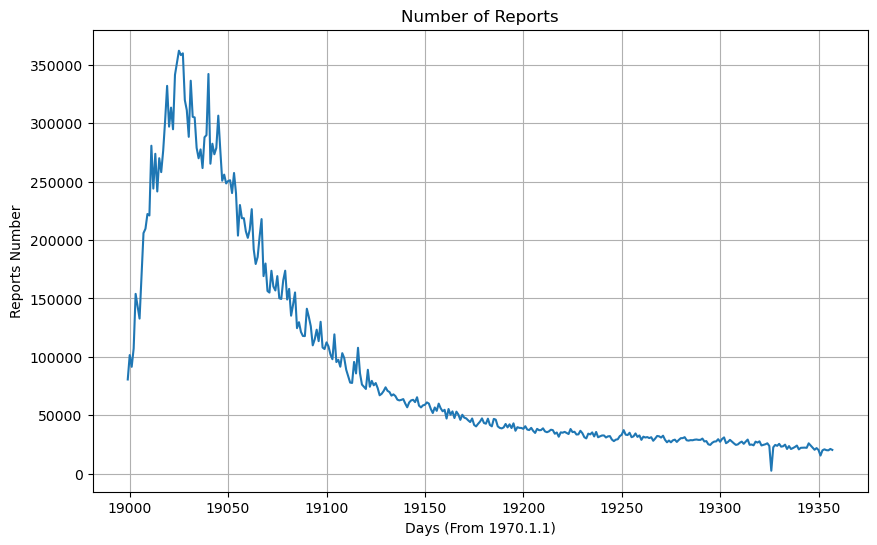
\includegraphics[width=.6\textwidth]{nr.png}
	\caption{number of reports with times}
	\label{img1}
\end{figure}

\subsection{Preprocessing}
First, for all experiments mentioned in this paper, data with columns containing outliers removed should be used. The outliers here are mainly words that do not conform to the rules of the Wordle game (e.g. words with a number of letters other than 5).

The data used for the training process must be relatively "smooth" for the ARIMA model to work well. We often use ADF (Augmented Dickey-Fuller) to verify the smoothness of the data, and use the difference method to eliminate the unsteadiness so that it meets the conditions needed for the ARIMA model. Figure 2 shows the image of the original data after one round of differencing.


\begin{figure}[H]
	\centering
	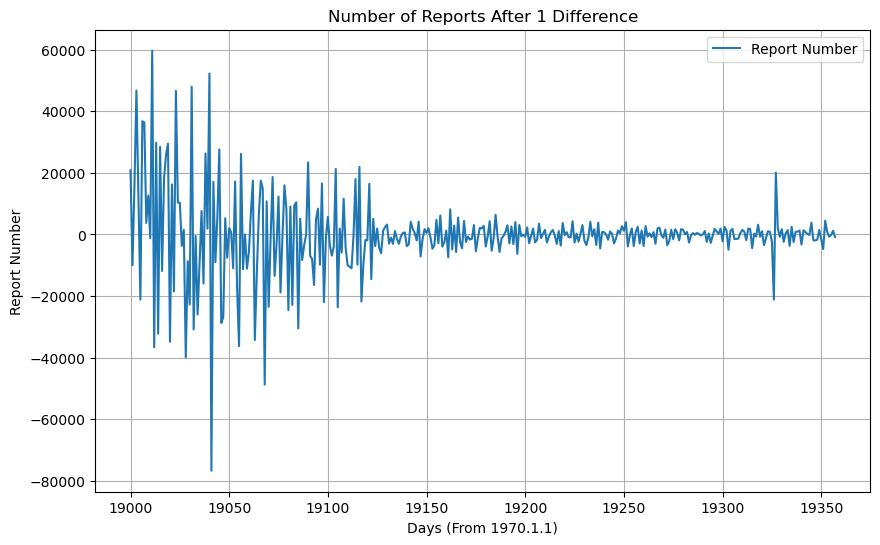
\includegraphics[width=.6\textwidth]{nra1d.png}
	\caption{number of reports after 1 difference}
	\label{img2}
\end{figure}

Comparing with Figure. 1, the overall trend of the data after one round of differencing is observed to be completely smooth. The results of the ADF validation (Table 2) show that the value of the ADF statistic is smaller than each critical value, so it indicates that the data after one round of differencing is smooth, and the ARIMA model can be used to predict the number of people reporting on a future day.
\begin{table}[!ht]
    \centering
    \begin{tabular}{|l|l|}
    \hline
        \textbf{Parameters} & \textbf{values} \\ \hline
        ADF statistic & -5.465670 \\ \hline
        p-value & 0.000002 \\ \hline
        Lags Used & 17 \\ \hline
        Number of observations & 336 \\ \hline
        Threshold 1 & -3.449963 \\ \hline
        Critical value 5 & -2.870181 \\ \hline
        Critical value 10 & -2.571373 \\ \hline
    \end{tabular}
	\caption{The results of ADF validation}
\end{table}


\subsection{Training}
The training is preceded by first partitioning the dataset. In order to calculate the generalization error and adjust the parameters, we divide the dataset into three parts: training, validation, and testing. First, the data set is partitioned into a 4:1 training set and a test set according to the hold out method, and then the training set is partitioned into a 4:1 training set and a validation set in the same way. In this way, the training set, validation set, and test set occupy 64\%, 16\%, and 20\% of the original data set, respectively. Among them, the test set is used to measure the generalization error and is not involved in training; the validation set is used to adjust the parameters to obtain the best model.

The error of the training model is described by the mean square error MSE.
\begin{equation}
E(D;f)=\frac1n\sum_{(x,y)\in D}(f(x)-y)^2
\end{equation}

where E denotes the mean square error; D denotes the dataset used for testing; f denotes the model obtained from training; f (x) is the y-value predicted by the model for x; and n is the size of D. A larger MSE means a worse model fit.

\subsection{Parameter selection}

The ARIMA model mainly consists of the AR (Autoregressive) model and MA (Moving Average) model. These two models require the selection of two main parameters.
\begin{itemize}
	\item The order p of the AR model, which is chosen by observing the partial autocorrelation function (PACF) plot.
	\item The order q of the MA model, which is chosen by observing the autocorrelation function (ACF) plot.
\end{itemize}
Plotting the ACF and PACF plots (figure 3), it is not difficult to find that both functions converge rapidly to flatness. In order to explore the best order choice, we search for the combination of p, q values that enter the plateau to find the set that minimizes the MSE of the model prediction validation set.
\begin{figure}[H]
	\centering    
	\subfigure[ACF]{				% 图片1([]内为子图标题)
		\label{fig:sub.roomhot}							% 子图1的标签
		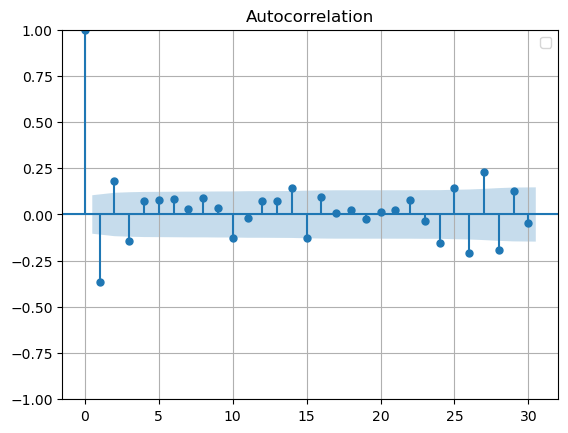
\includegraphics[width=0.3\textwidth]{acf.png}}% 子图1的相对位置
	\subfigure[PACF]{				% 图片2
		\label{fig:sub.floorhot}						% 子图2的标签
		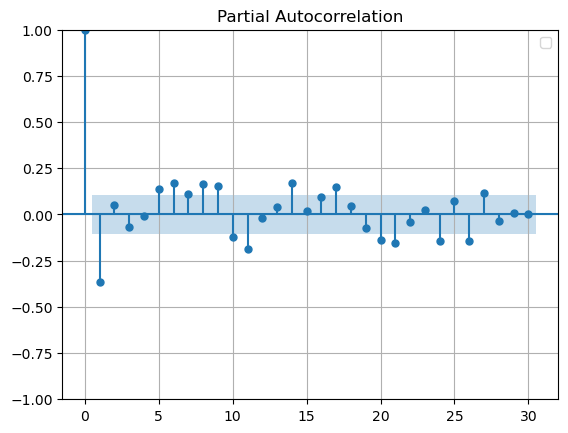
\includegraphics[width=0.3\textwidth]{pacf.png}}% 子图2的相对位置
	\caption{ACF and PACF plots}		% 总图标题
	\label{img3}									% 总图标签
\end{figure}
The thermal diagram of the MSE for each combination of parameters tested is shown in the figure 4.
\begin{figure}[H]
	\centering
	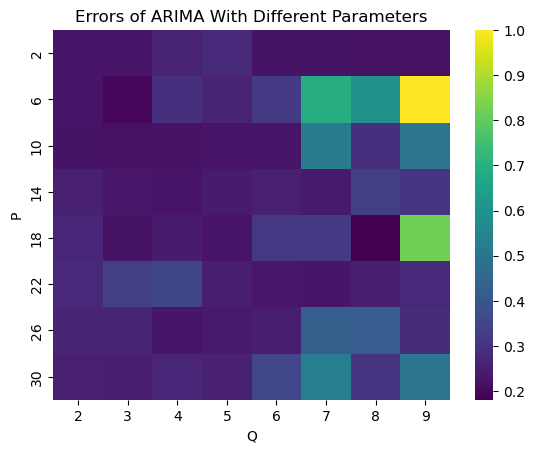
\includegraphics[width=.6\textwidth]{erhmp.png}
	\caption{Heat map of MSEs}
	\label{img4}
\end{figure}

The optimization method used here is \textbf{innovations mle}, and the training results prove that this optimizer converges most easily to obtain the most effective parameter combinations. As shown in the figure, the parameter combination with the smallest standard deviation is $p=18,q=8$.

In summary, the predicted data are obtained after the inverse difference of the prediction results. 27,540 people are predicted to report on March 1, 2023; there is 90\% confidence that the number of people reporting on that day is between [0, 49485](figure 5).

\begin{figure}[H]
	\centering
	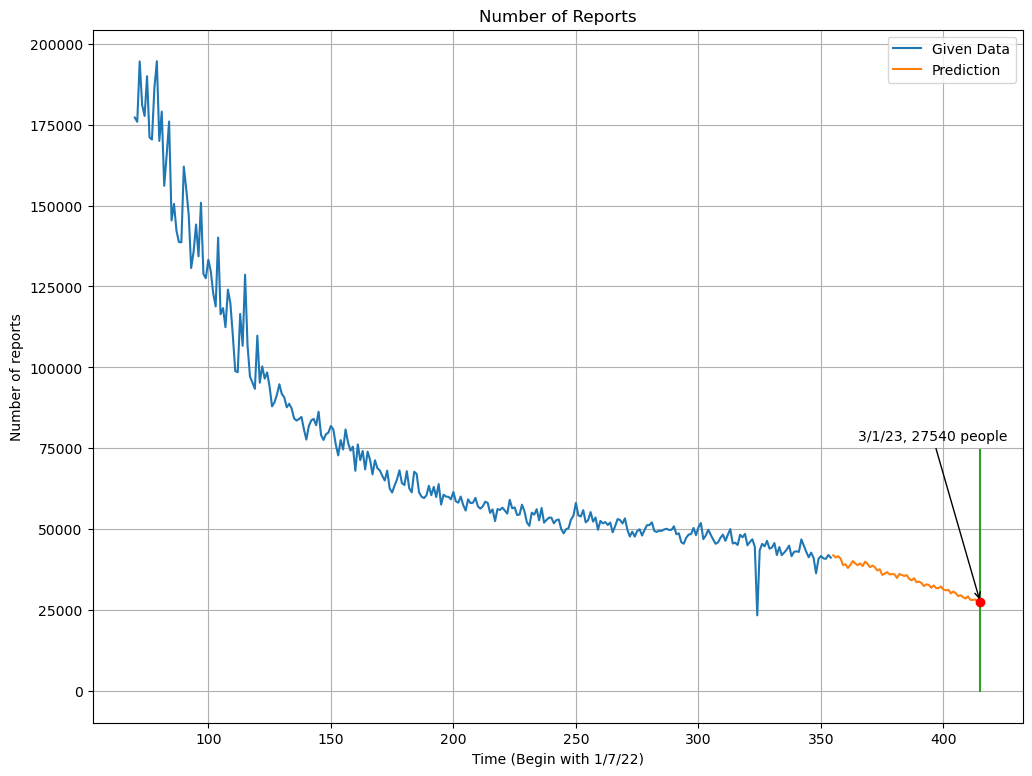
\includegraphics[width=.6\textwidth]{prd.png}
	\caption{final result}
	\label{img5}
\end{figure}

\subsection{Model Analysis}
Using the most suitable combination of parameters obtained from the measurement, it is used for the test set to measure the generalization error. Since we took one difference, we used it as a test set after one difference to test it and obtained its generalization error MSE as $1.499\times 10^7$. As shown in the figure 6, except for individual outliers, the ARIMA model still has a predictive effect on this kind of data with strong local fluctuations.
\begin{figure}[H]
	\centering    
	\subfigure[Global]{				% 图片1([]内为子图标题)
		\label{fig:sub.roomhot4}							% 子图1的标签
		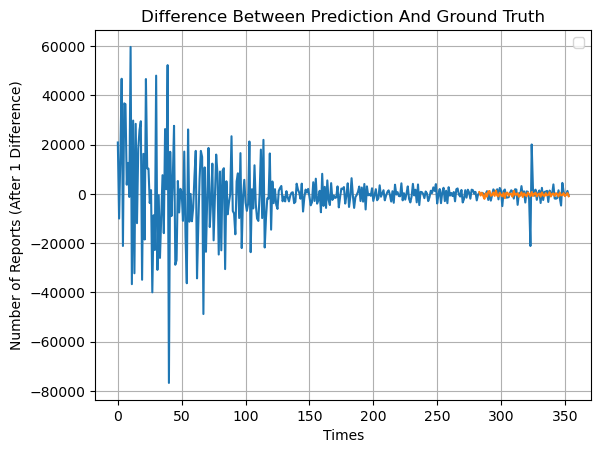
\includegraphics[width=0.5\textwidth]{ARIMA1.png}}% 子图1的相对位置
	\subfigure[Local]{				% 图片2
		\label{fig:sub.floorhot4}						% 子图2的标签
		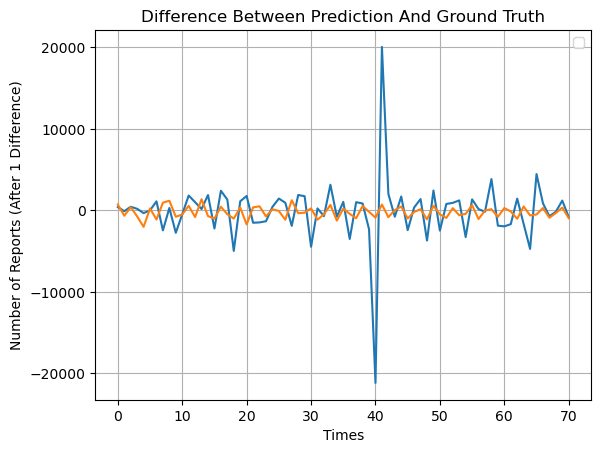
\includegraphics[width=0.5\textwidth]{ARIMA2.png}}% 子图2的相对位置
	\caption{prediction data with origin data}		% 总图标题
	\label{img34}									% 总图标签
\end{figure}

In addition, because of the insufficient data in the dataset, it is not enough to make the model converge for all combinations of parameters involved in the test. It is also possible to consider collecting more datasets or using more advanced training methods to obtain better results.

As explained in the previous section, the date and word itself affect the distribution of wordle players' attempts (or the distribution of scores), so we can try to build a model to predict the proportion of players with each score using each feature of the date and word.

\section{Task2: Correlation Analysis}

The correlation between the percentage of each score and the mean as well as the standard deviation is strongly related, and the correlation between the word features and the percentage can be obtained by correlation analysis of the word features as well as the mean and standard deviation.

\subsection{Calculation Method Selection}

We used the correlation coefficient to represent the two-by-two relationship between the four word indicators of word frequency, MNRL, root word, and word nature and the mean and standard deviation of the number of attempts.

Since the mean and standard deviation of the number of attempts are continuous data, and the four word indicators are not uniformly continuous or not, in order to calculate the correlation coefficients between the data as accurately as possible, we adopted two different calculation methods: ANOVA and Spearman's correlation coefficient.

For the three features of MNRL, word roots, and word properties, whose are all discrete indicators, we chose to use ANOVA.

For the continuous type of word frequency, we chose to use Spearman's correlation coefficient or Pearson's correlation coefficient for evaluation.


\subsection{Calculation Results and Analysis}

As an example: MNRL has two classifications, 1 and 2, and we extract the mean and standard deviation of the number of attempts corresponding to each of them. The variance of these two consecutive values is calculated. A t-test can be used to calculate the t-value and the p-value. (The t-value can be a standardized measure of the difference in means between two groups of data, and the p-value indicates a statistic for the significance of the t-test results, with the p-value pre-set at 0.05 and less than 0.05 indicating a significant difference)

Table.\ref{tab:tdata} and Table.\ref{tab:pdata}are the ANOVA results for these three indicators and two continuous-type indicators.

\begin{table*}
	\centering
	\begin{tabular}{  |c|c|c|c|
		}
		
		\hline
		T-value 	& MNRL	& root	 & character \\ 
		\hline
		Means	& -7.14		& -0.66		 & -0.96  \\ 
		\hline 
		Stddev & 1.921 		& -0.77		 & -0.56  \\ 
		\hline 
		
	\end{tabular}
	\caption{T-value data}
	\label{tab:tdata}
\end{table*}

\begin{table*}
	\centering
	\begin{tabular}{  |c|c|c|c|
		}
		
		\hline
		P-value 	& MNRL	& root	 & character \\ 
		\hline
		Means	& 0.00  &  0.51 & 0.49 \\ 
		\hline 
		Stddev & 0.06 & 0.44 & 0.55  \\ 
		\hline 
		
	\end{tabular}
	\caption{P-value data}
	\label{tab:pdata}
\end{table*}
By observing the data in the above table, we can find that the two indicators of word root and word nature have little relationship with the mean value of the number of attempts and the standard deviation, while Means is highly correlated with the values of MNRL, and Stddev is not significantly correlated with MNRL.

We calculated the $\mu$ and $\sigma$ values for different values (1 and 2) of Means in MNRL, and the results are as follows.
\begin{table*}
	\centering
	\begin{tabular}{  |c|c|c|
		}
		
		\hline
		$\mu$ 	& MNRL=1 & MNRL=2 \\ 
		\hline
		Means	& 4.10  &  4.42 \\ 
		\hline 
		
	\end{tabular}
	\caption{Means' $\mu$  of different MNRL}
	\label{tab:miu}
\end{table*}

\begin{table*}
	\centering
	\begin{tabular}{  |c|c|c|
		}
		
		\hline
		$\sigma$ 	& MNRL=1 & MNRL=2 \\ 
		\hline
		Means	& 0.37  &  0.38 \\ 
		\hline 
		
	\end{tabular}
	\caption{Means' $\sigma$ of different MNRL}
	\label{tab:sigma}
\end{table*}

We can find that the Means values for different values of MNRL vary widely, and the standard deviations are small and similar in the same category; we can thus conclude how MNRL affects the average number of attempts: when MNRL is 1, the average number of attempts is 4.10, and when it is 2, the average number of attempts is 4.42. This shows that the difficulty increases significantly.

The following is the basis for the choice of Spearman and Pearson to see if the linear relationship as well as the normal distribution is met.

To visualize Frequency-Means as well as Frequency-Std.

\begin{figure}[H]
	\centering    
	\subfigure[Mean]{				% 图片1([]内为子图标题)
		\label{fig:sub.roomhot5}							% 子图1的标签
		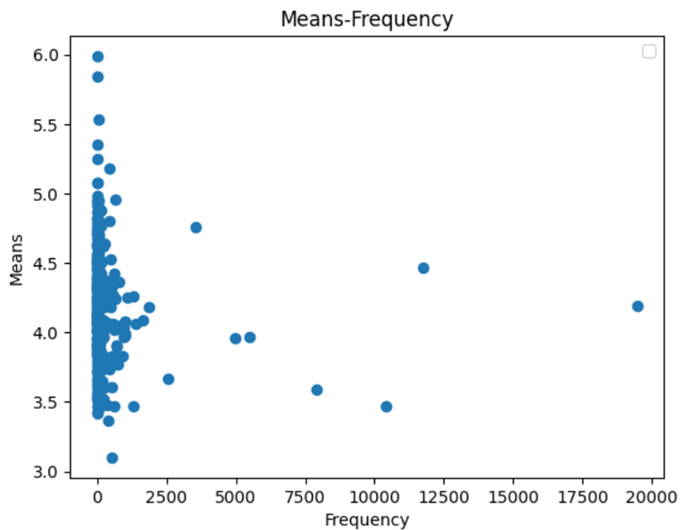
\includegraphics[width=0.5\textwidth]{Frequency-Means.png}}% 子图1的相对位置
	\subfigure[Std]{				% 图片2
		\label{fig:sub.floorhot5}						% 子图2的标签
		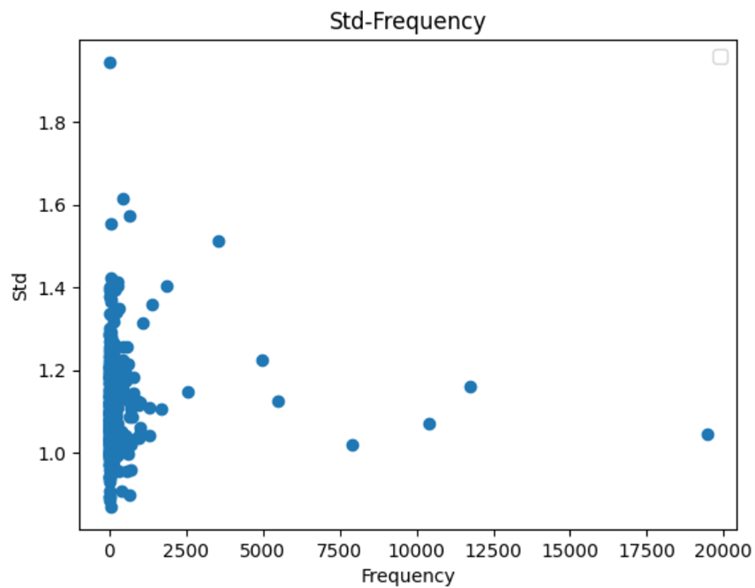
\includegraphics[width=0.5\textwidth]{Frequency-Std.png}}% 子图2的相对位置
	\caption{Frequency with *}		% 总图标题
	\label{img35}									% 总图标签
\end{figure}


It is found that there is no linear relationship between Frequency-Means as well as Frequency-Std.

In the following, we have made Q-Q plots for Means, Std, and Frequency to determine whether the three indicators conform to a normal distribution by comparing the quartiles of the three indicators with the quartiles of the expected distribution.

\begin{figure}[H]
	\centering
	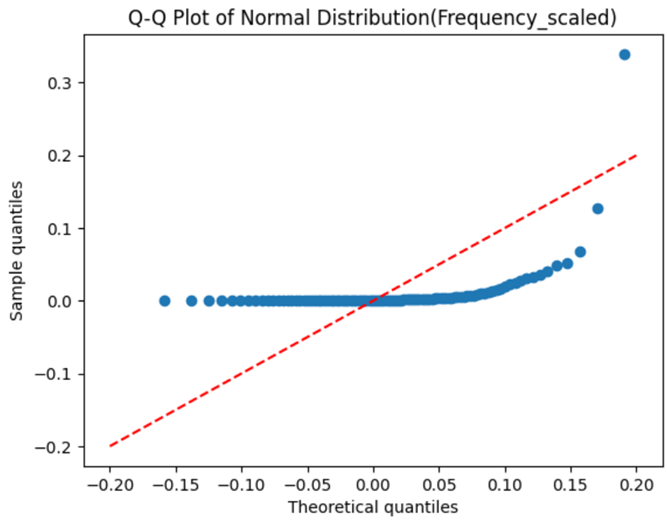
\includegraphics[width=.6\textwidth]{Freq-QQ.png}
	\caption{Frequency-QQ}
	\label{img22}
\end{figure}

By visual observation, Frequency did not conform to the normal distribution.

Based on the above two factors, we found that the premise of Pearson correlation coefficient calculation was not satisfied, so we chose to use Spearman correlation coefficient for calculation.

We can calculate Spearman correlation coefficients and p-values of word frequencies with Means and Stddev, respectively, by sorting each indicator from smallest to largest and calculating the position difference as well as the sum of position differences after sorting, as follows.
\begin{table*}
	\centering
	\begin{tabular}{  |c|c|c|
		}
		
		\hline
		Spearman correlation coefficient 	& Means & Stddev \\ 
		\hline
		Frequency	& -0.018  &  -0.044 \\ 
		\hline 
		
	\end{tabular}
	\caption{Spearman correlation coefficient}
	\label{tab:Spearson-f}
\end{table*}

\begin{table*}
	\centering
	\begin{tabular}{  |c|c|c|
		}
		
		\hline
		P-value 	& Means & Stddev \\ 
		\hline
		Frequency	& 0.742  &  0.407 \\ 
		\hline 
		
	\end{tabular}
	\caption{P-value}
	\label{tab:Spearman-f-p}
\end{table*}
By evaluating the observation of the above four indicators, we can conclude that word frequency has little relationship with the mean as well as the standard deviation of the number of attempts.


\section{Task 3: Predicting the distribution of player attempts}
Since the sum of the player shares for each score must be 100\%, it would be difficult to satisfy this feature if the player shares for all 7 attempts were predicted by the model. However, we note that if we fit the 7 player categories with a probability density function, we can avoid this problem by using the model to predict only the probability density function. We decided to first fit the relationship between the number of attempts and the percentage using a probability density function of a probability distribution model, and then use the parameters of that probability distribution model (e.g., mean and variance of the Gaussian distribution; $\lambda$ of the Poisson distribution; degrees of freedom of the chi-square distribution, etc.) to determine the probability density function. After that, the problem is reduced to predicting these parameters using time and word features, and then using these parameters to determine the probability density function as a fitting function for the number of attempts and the percentage of players to calculate the percentage, without having to consider that the sum of the percentages must be 100\%. The schematic is shown in Figure 9.

\begin{figure}[H]
	\centering
	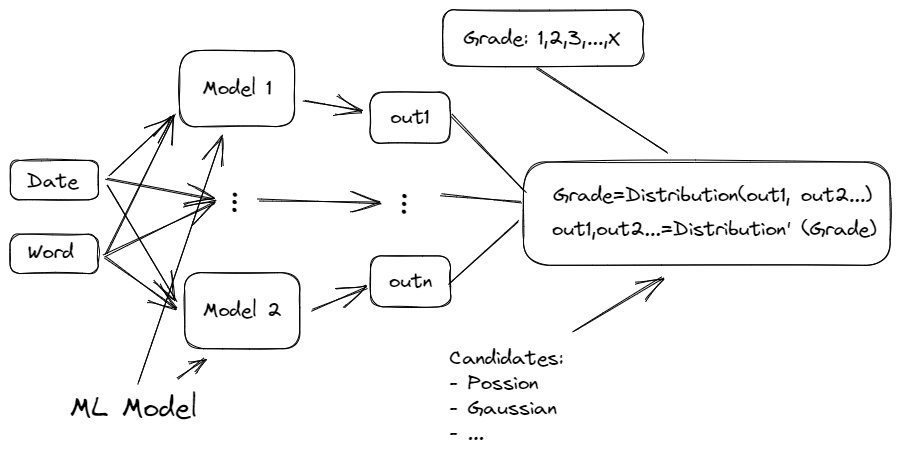
\includegraphics[width=.9\textwidth]{mcm.excalidraw.png}
	\caption{Model structure}
	\label{img8}
\end{figure}

Next we need to:
\begin{itemize}
	\item Select a suitable probability distribution model.
	\item Establish the parameters for predicting the probability distribution model with date and word features, and confirm the probability density function used for the fit.
\end{itemize}

\subsection{Choosing Probability Distribution Model}
\subsubsection{Model}
In the data set, we can calculate the mean and standard deviation of the number of attempts for each word, which we think is of great significance for the percentage of attempts.
	
The normal distribution is an important continuous-type probability distribution that is widely found in nature and social phenomena. For example, the distribution of students' grades and the distribution of players' game scores are typical examples of normal distributions. In the context of Wordle game, we can consider the number of attempts of a player as the score of the game.

Then if the scores of Wordle are continuous, we can assume that the scores of the game satisfy the normal distribution very well.
	However, the game's score (number of player attempts) has only 7 values (1 try, 2 tries, 3 tries, 4 tries, 5 tries, 6 tries, and more than 7 tries), which does not meet the requirements of a normal distribution with continuous data. So we chose to use the discrete normal distribution model [1], where the percentage of a certain number of tries can be found by integrating over the probability interval.
	The specific process is as follows.
We first establish a function of normal distribution for each data by taking the mean ($\mu$) and standard deviation ($\sigma$) of the number of player attempts for each data as parameters.
% (正态分布方程 !!!!!!!!!!!!!!!)  
\begin{equation}
	f(x)=\frac{1}{\sqrt{2\pi}\sigma}\exp(-\frac{(x-\mu)^2}{2\sigma^2})
\end{equation}
At this point, if we want to find the percentage of player attempts for x (1<=x<=7), we can integrate the probability function x-0.5 to x+0.5 for this interval with the following formula.
% (积分方程 !!!!!!!!!!)  
\begin{equation}
	\frac{1}{\sqrt{2\pi}\sigma}\int^{x+0.5}_{x-0.5}e^{-\frac{(t-\mu)^2}{2\sigma^2}}dt
\end{equation}
In order to verify the applicability of the discrete normal distribution model in the context of this problem, we validated the discrete normal distribution model with data from the dataset. The results performed well, and some of the results are shown below.

\begin{figure}[H]
	\centering    
	\subfigure[]{				% 图片1([]内为子图标题)
		\label{fig:sub.roomhot3}							% 子图1的标签
		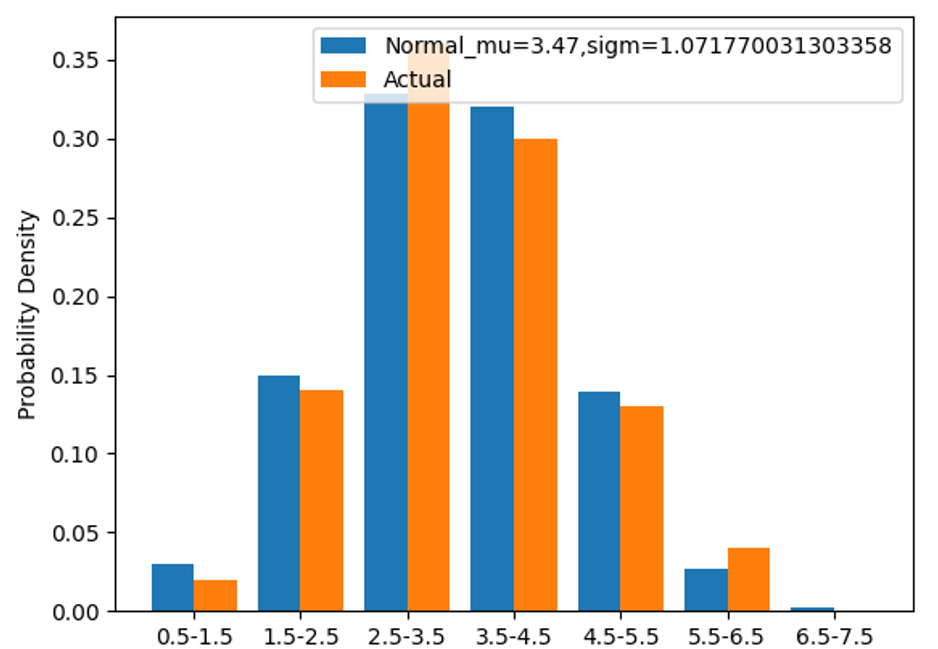
\includegraphics[width=0.3\textwidth]{nm act.png}}% 子图1的相对位置
	\subfigure[]{				% 图片2
		\label{fig:sub.floorhot3}						% 子图2的标签
		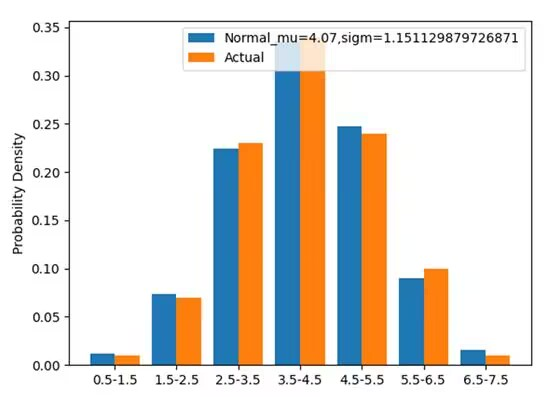
\includegraphics[width=0.3\textwidth]{nm act2.jpg}}% 子图2的相对位置
	\caption{some typical results}		% 总图标题
	\label{img33}									% 总图标签
\end{figure}
% 全部图形的链接为:(!!!!!!!!!)


\subsection{Building a predictive model} 
As above, we still visualize the relationship between time and word features and the two dependent variables. Here the data is pre-processed, i.e. z-score normalized and projected to between 0 and 1. As in Figure 11.
\begin{figure}[H]
	\centering
	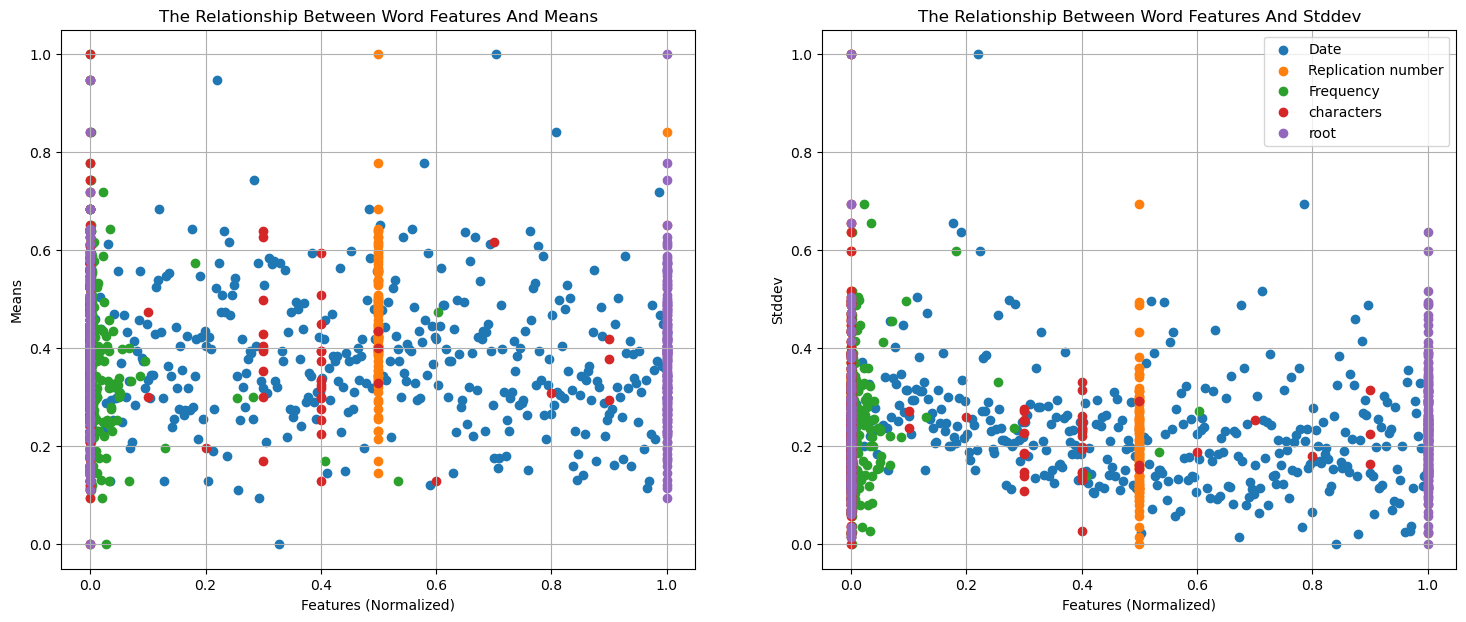
\includegraphics[width=.6\textwidth]{rbfms.png}
	\label{img30}
	\caption{scatter map (normalized)}
\end{figure}
As the figure shows, there is no particular reason driving us to choose the particular model. Therefore we still use linear regression to do the prediction work. However, at this point there is still some correlation between these features, so we first processed the data with principal component analysis (PCA) to obtain 5 principal components. Since there are not many features, all principal components can be retained for the next step. After PCA, the correlation between principal components was minimal.
The data set was still partitioned as in the previous section, and a linear regression model was fitted and trained for both variables using the linear regression model. The generalization errors on the test set were measured as in Table 9.
\begin{table}[!ht]
    \centering
    \begin{tabular}{|l|l|l|}
    \hline
        \textbf{} & \textbf{Mean} & \textbf{Standard deviation} \\ \hline
        \textbf{MSE} & 0.434763 & 0.008357 \\ \hline
        \textbf{MAE} & 0.453589 & 0.072288 \\ \hline

    \end{tabular}
	\caption{MSE \& MAE}
\end{table}
The fitting effect is shown in Figure 12.
\begin{figure}[H]
	\centering
	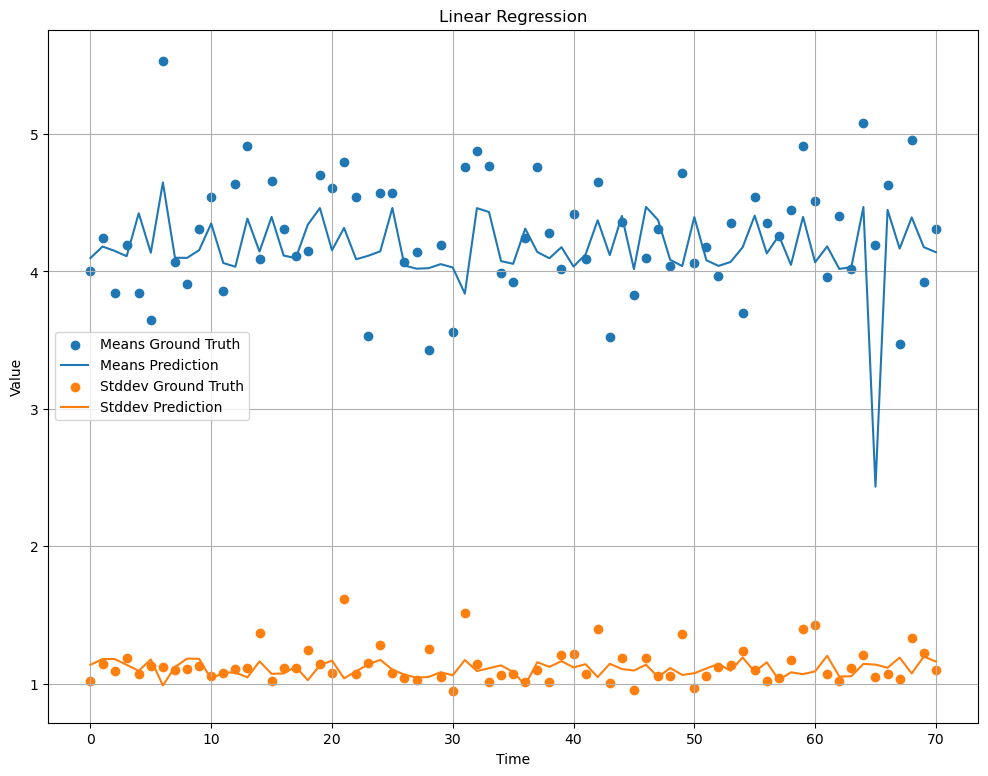
\includegraphics[width=.6\textwidth]{pms.png}
	\label{img31}
	\caption{fit result}
\end{figure}

\subsection{Model solving}
	After testing this discrete normal distribution model, we verified its validity. We can make predictions about the percentage of player attempts for a word at a future date. For example, the prediction is made for the case of March 1, 2023, when the word is eerie. We first use the mean and standard deviation of the number of player attempts calculated by Task3 to input into this model, and the final result is calculated as follows.
 \begin{figure}[H]
	\centering
	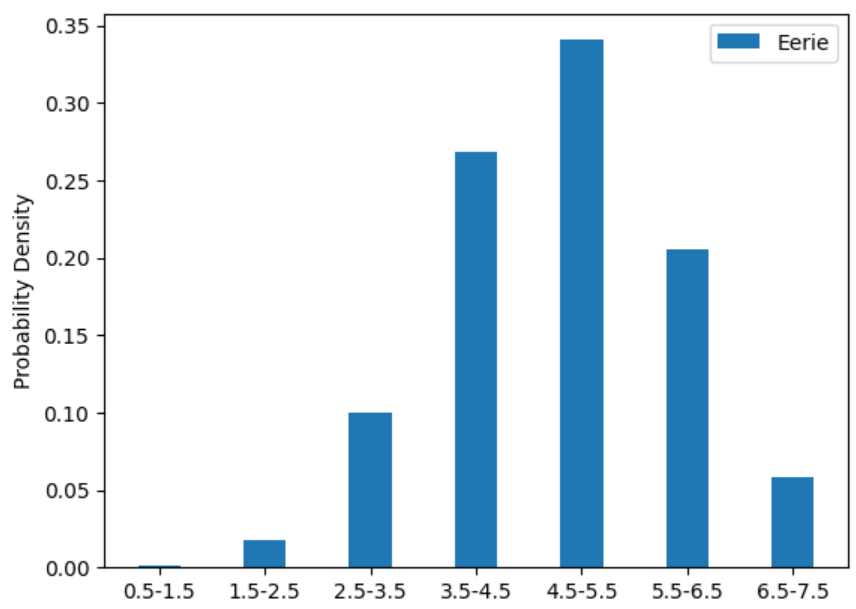
\includegraphics[width=.6\textwidth]{eerie.png}
	\caption{the distribution of player tries of word "eerie"}
	\label{img10}
\end{figure}

\subsection{Model analysis}
\textbf{Disadvantages Analysis}:The model we built has certain uncertainties, which are mainly reflected in the following aspects. One, we use time as well as four indicators of words as factors affecting the number of player attempts, and these indicators may not be comprehensive, leading to an inaccurate model. Second, the word frequency indicators of words are sourced from major corpora, which are mostly old, and words from recent times may not be counted, resulting in the indicator not being time-sensitive.

\textbf{Merit analysis}:
We chose the indicator of the number of repeated letters in words, and this indicator has a large impact on the final results. This indicator has some practical significance. In the Wordle game, if there is a word in the wrong place, we do not know how many letters are present in the answer. If there are more than one letter, this makes the game much more difficult and leads to a corresponding increase in the number of attempts. Therefore, we have a high degree of confidence in our model.

\section{Task 4: Classifying word difficulty}
\subsection{Hierarchical clustering-based word difficulty classification model}
\subsubsection{Indicator selection}
To analyze their word properties, we screened four indicators of word frequency, MNRL, root, and wordiness as the basic features to classify the difficulty of words, and referred to the commonly used Gutenberg corpus, Brown corpus, Reuters corpus, WordNet corpus, and treebank corpus to count the word frequency, MNRL, root, and wordiness of each historical answer word in wordle The word frequency, MNRL, root word, and lexical property of each historical answer word in wordle were calculated. The following is a specific analysis of these four word attributes.

\begin{enumerate}
	\item Word frequency: how often a word is used in people's social life. This indicator reflects how common the word is. In general, if a word has a smaller word frequency, it can be considered as more difficult.
	\item MNRL: The number of repeated letters in a word. Generally, if there are more than one letter in a word, it will make the word difficult to be guessed.
	\item Root: The presence or absence of a root word in a word. In terms of historical experience, words with roots are generally more common in ordinary life and can be assumed to be less difficult to guess.
	\item Word nature: The nature of a word such as a noun, verb, etc. The lexical nature of different words can reflect the different difficulty of the word. Generally, verbs and prepositions are more common in life, and words with these lexical natures can be considered less difficult.
\end{enumerate}

In summary, the above 4 attributes can basically reflect the difficulty level of words, and can be used as part of the criteria for classifying the difficulty of words.

\subsubsection{Data pre-processing}

By analyzing the dataset of the four indicators of each historical answer word, the ranges of each indicator are very different and do not belong to the same scale, and the range of word frequency indicators fluctuates greatly, which may have some influence on the final result of dividing the difficulty, so we decided to standardize the dataset.

Here, the maximum-minimum normalization is adopted to pre-process the data set, and the interval is scaled to the range of 0 to 1, which is convenient for the later hierarchical clustering to divide the word difficulty problem.

\subsubsection{Model building}

To classify the word difficulty based on the index dataset of words, here we establish a word difficulty classification model based on hierarchical clustering and finally get the criteria for determining the classification of word difficulty.

Considering that hierarchical clustering does not require a pre-determined number of clusters for clustering, and is suitable for data sets with a small amount of data, and can handle noise and outliers, in line with our data set, the cohesive hierarchical clustering model using hierarchical clustering is used, and the clustering is performed from the bottom up, gradually merging into larger and larger clusters, and similar data points are merged until certain stopping conditions are met.

\begin{figure}[H]
	\centering
	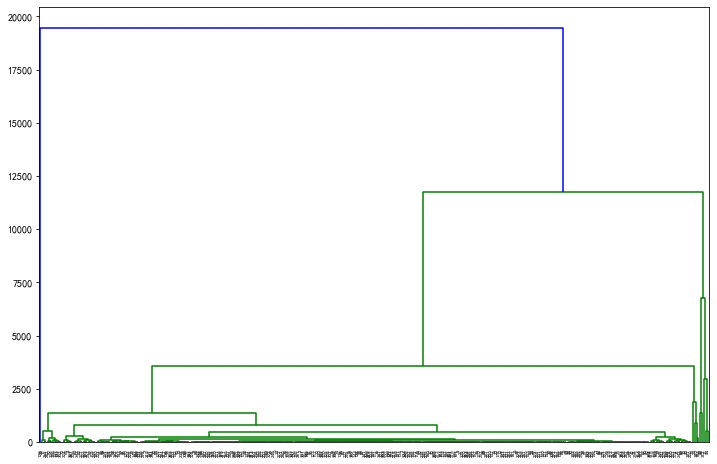
\includegraphics[width=.6\textwidth]{pic1.png}
	\caption{hierarchical clustering diagram}
	\label{img13}
\end{figure}
%\begin{figure}[H]
%    \centering
%    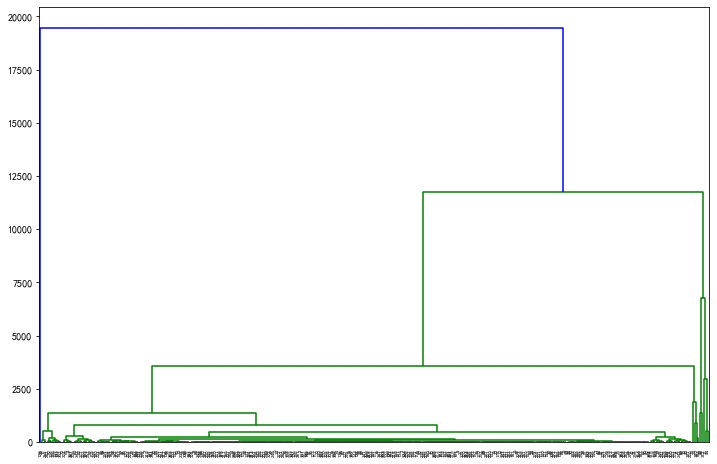
\includegraphics[width=.7\textwidth]{pic1.png}
%    \caption{Some change in eigenvalues}
%    \label{img}
%\end{figure}

In the hierarchical clustering process, cosine similarity was used as the distance measure to maximize the farthest distance between clusters as the connection method of clustering. The metrics in the dataset were hierarchically clustered, and the analysis showed that the contour coefficient was highest when k=2, i.e., when clustered into 2 classes, and this clustering was considered the best, and clustering into 2 classes was more consistent with the classification of word difficulty.
The contour coefficient is calculated as follows.
For the ith sample, let a(i) be its average distance from other samples in the same cluster, and b(i) be its average distance from all samples in the nearest other clusters (i.e., the average distance between clusters), then the contour coefficient of this sample is:

\begin{equation}
	s(i)=(b(i)-a(i)) / \max \{a(i), b(i)\}
\end{equation}

The contour coefficient of the whole data set is the average of the contour coefficients of all samples. A larger value of the contour coefficient represents a better result of clustering.
The following is a comparison of the contour coefficients for different k values.

\begin{table}[hbp]
	\centering
	
	\label{tab:pagenum}
	\begin{tabular}{lllll}
		\toprule
		k& 2 & 3 & 4 \\
		\midrule
		Contour factor  & 0.9688079418026865 & 0.9584611141643063 & 0.9490023468641484\\
		
		\bottomrule
	\end{tabular}
	\caption{comparison of the contour coefficients for different k values}
\end{table}

\subsubsection{Model solving and result display}

1.Hierarchical clustering to classify word difficulty results

When the clustering with a k value of 2 was initially determined to be good, we selected 2 classes for specific clustering exploration, indicated different labels for all words, and initially delineated the word difficulty as 2 difficulties. In order to delineate the specific difficulty determination criteria, the word data with different labels indicated earlier are grouped according to different two classes of labels, and the mean value of each word attribute after the grouping is sought, and the obtained mean value is taken as its clustering center of mass, and its center of mass features are analyzed, and the word difficulty can be divided into easy-to-guess word class and hard-to-guess word class.

The easy-to-guess word class is for words with larger MNRL values and more word frequency, and the hard-to-guess word class is for words with smaller MNRL values and less word frequency. The following is the data of the center of mass after clustering.

\begin{table}[hbp]
	\centering
	
	\label{tab:pagenum}
	\begin{tabular}{lllll}
		\toprule
		& MNRL & word frequency & Morpheme & root of word \\
		\midrule
		Classification 1  & 1.80315 & 628.669291 & 1.346457 & 0.503937\\
		\midrule
		Classification 2  & 1.00000 & 135.671053 & 0.000000 & 0.508772\\	
		\bottomrule
	\end{tabular}
	\caption{comparison of the contour coefficients for different k values}
\end{table}

2.Visualization of clustering results

In order to present the results better and observe whether the results are obvious after clustering, a three-dimensional visualization is drawn here, where the three coordinates correspond to the three word attributes of word frequency, MNRL, and lexicality, respectively. The blue dots indicate one category after clustering, and the red dots indicate the other category. 	It can be seen that there are obvious boundaries between the two colors of points, and the blue points are mostly clustered in one category and the red points are clustered in one category, which can indicate good clustering effect.

The specific three-dimensional image after clustering is shown as follows.
\begin{figure}[H]
	\centering
	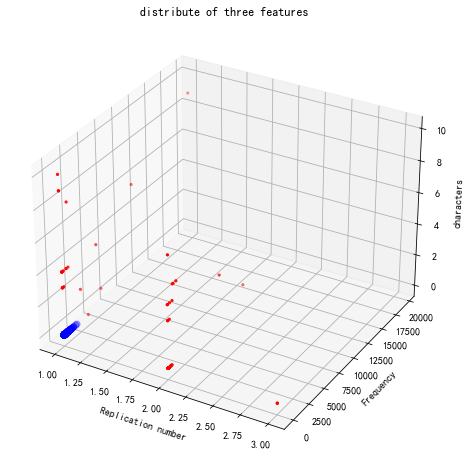
\includegraphics[width=.6\textwidth]{pic2.png}
	\caption{distributions of features}
	\label{img14}
\end{figure}
\begin{figure}[H]
	\centering
	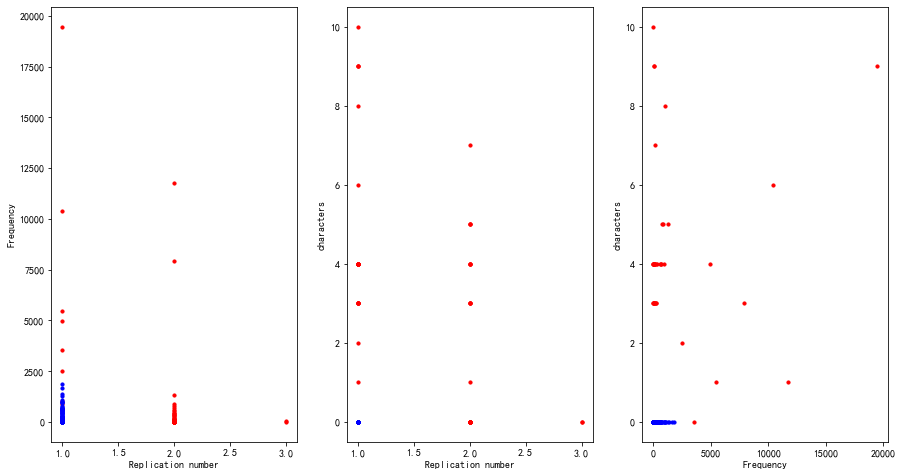
\includegraphics[width=.6\textwidth]{pic3.png}
	\caption{distributions of each 2 features}
	\label{img15}
\end{figure}
The two-dimensional diagrams of the respective two classes after clustering are as follows.

After clustering, the different two categories of difficulty categories are aggregated and the numerical categories of the three attributes of the words are as follows.
\begin{figure}[H]
	\centering
	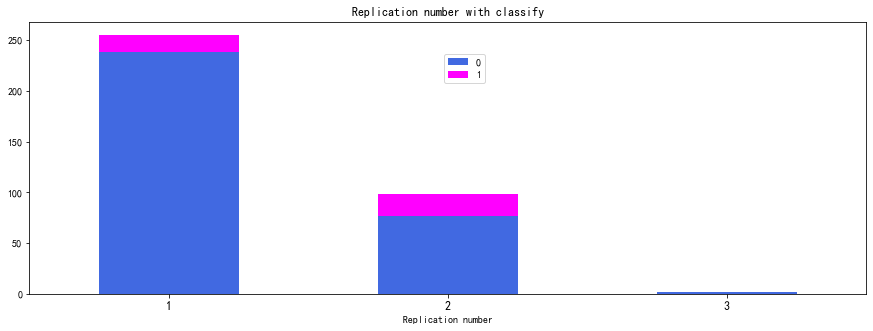
\includegraphics[width=.8\textwidth]{pic4.png}
	\caption{classifications of 3 features 1}
	\label{img16}
\end{figure}
\begin{figure}[H]
	\centering
	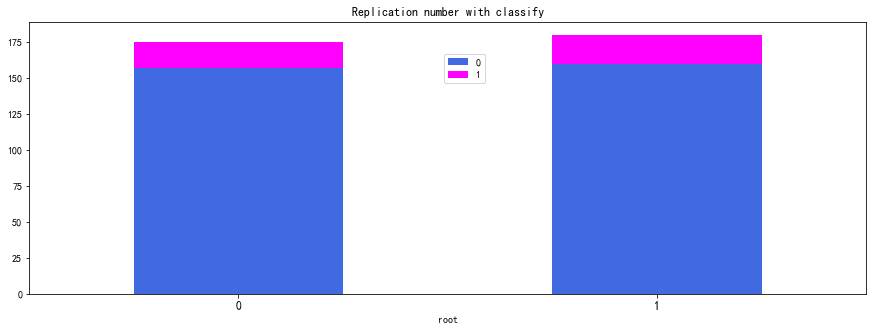
\includegraphics[width=.8\textwidth]{pic5.png}
	\caption{classifications of 3 features 2}
	\label{img17}
\end{figure}
\begin{figure}[H]
	\centering
	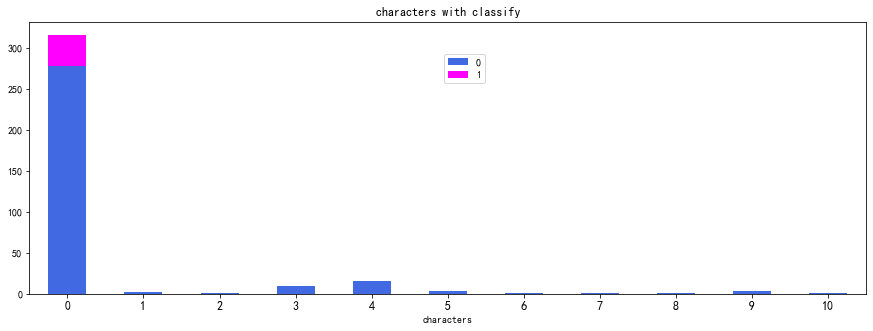
\includegraphics[width=.8\textwidth]{pic6.png}
	\caption{classifications of 3 features 3}
	\label{img18}
\end{figure}
3.Finding the contribution of each word index to the clustering results based on the WSS formula

After getting the results after clustering, for each indicator, calculate the sum of variance in different levels of clustering, that is, calculate the sum of variance of the indicator in different clusters after clustering, and then divide it by the total variance to get the contribution degree of the indicator.

\begin{equation}
WSS=\Sigma\|x i-c\|^{\wedge} 2(i=1,2, \ldots, n)
\end{equation}

Finally, the contribution of each respective metric in the total metric is shown in a fan chart based on the contribution of the obtained metrics, with MNRL and word frequency contributing the most to the clustering results, visualized as follows.
\begin{figure}[H]
	\centering
	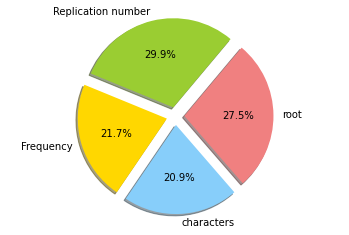
\includegraphics[width=.6\textwidth]{pic7.png}
	\caption{number of reports with times}
	\label{img19}
\end{figure}

\subsection{Support vector machine based specific word difficulty classification model} 

\subsubsection{Delineating the training test set and data preprocessing}

In order to classify the new answer words into one of the two classes obtained from the previous as well as the clustering, a suitable classification model learner must be selected to fit the training to each word attribute and classification label.
First, a simple cross-validation of the dataset should be performed first by selecting a training set and a test set according to a given ratio, with the number of training and test sets being 8:2.

In terms of data preprocessing, maximum-minimum normalization is used, and the specific steps are described in the above model as well as, so we will not go into too much detail here.

\subsubsection{Model Building}

Among many classification learning models, here we choose support vector machine classifier, which is a powerful classifier for linear and nonlinear classification problems and can handle high-dimensional data and data sets with small sample size, which is more suitable for the characteristics of our data set, 4-dimensional data and small data sample size. In addition, it can also handle classification problems well and can prevent overfitting by regularization terms.

\subsubsection{Model Solving and Results Presentation}

1.Support vector machine classification of specific word difficulty

The support vector machine was selected to classify the specific word difficulty, and the following specific tuning parameters were used to violently search the parameters using the grid search method to determine the specific suitable parameters to make the best accuracy of the classification prediction results.
Through the grid search method, the penalty parameter is determined to be 3. When the penalty parameter is larger, it can make the classifier more mainly classify correctly, and the number of control polynomial kernel functions is 3. The polynomial kernel function type is polynomial kernel function, which can map the feature space into a high-dimensional polynomial space and can handle some nonlinear classification. After tuning the parameters, the accuracy of the initially obtained classification model is close to 1. The test set and the prediction set can 	Basically match, which indicates that the classification effect is good.
For the new word EERIE classified with the trained classification model, the classification result obtained is 1, i.e., it can be classified as a class of hard-to-guess words.

2.Determining the accuracy of the classification model

In order to determine the specific accuracy of the classification model, four metrics are used here to determine the accuracy of the classification model, namely precision, recall, F1 value and support.

\begin{enumerate}
	\item Precision: the percentage of samples with positive predictions that are actually positive cases.
	\item Recall: The percentage of samples with positive cases that are predicted to be positive cases.
	\item F1 value: The summed average of precision and recall.
	\item Support: the number of samples per category in the true label.
	The specific accuracies are listed in the following table:
\end{enumerate}

\begin{table}[hbp]
	\centering
	
	\label{tab:pagenum}
	\begin{tabular}{lllll}
		\toprule
		& precision &  recall & f1-score & support \\
		\midrule
		Classification 1  & 1.00 & 1.00 & 1.00 & 22\\
		\midrule
		Classification 2  & 1.00 & 1.00 & 1.00 & 49\\	
		\bottomrule
	\end{tabular}
	\caption{comparison of the contour coefficients for different k values}
\end{table}


\section{Task 5: Interesting Characteristics of The Dataset}
We also conducted data exploration of the dataset and found some interesting characteristics.

First, we found that the number of reports of playing difficult mode as a percentage of reports slowly decreases as the total number of reports increases, and the trend is clear (as shown in the figure 11). Because a game has a relatively limited long-term audience, it does not simply increase with the number of players.
\begin{figure}[H]
	\centering
	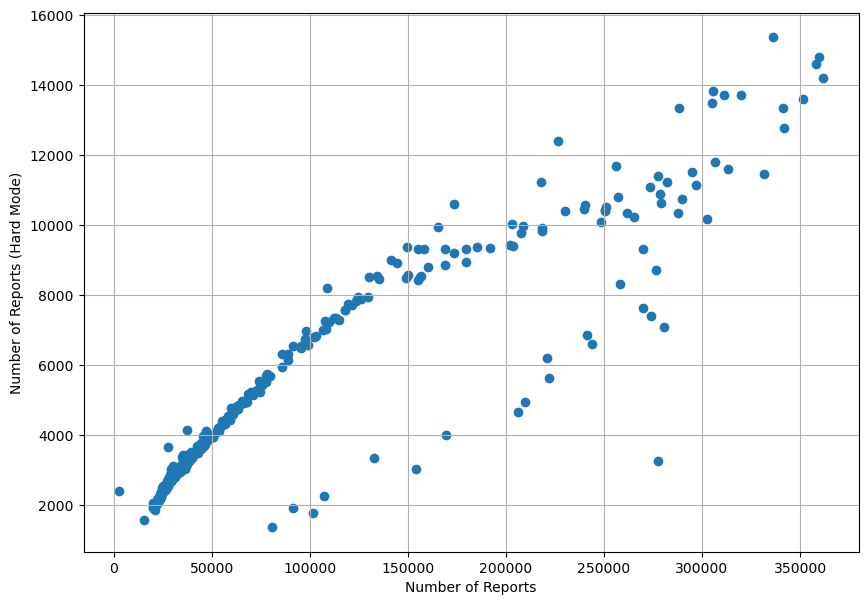
\includegraphics[width=.6\textwidth]{rhr.png}
	\caption{}
	\label{img11}
\end{figure}

Second, we calculated the mean and variance of the player scores, and found that both obeyed a normal distribution according to their qq plots. Both are shown in Figure 22.
\begin{figure}[H]
	\centering    
	\subfigure[Mean]{				% 图片1([]内为子图标题)
		\label{fig:sub.roomhot1}							% 子图1的标签
		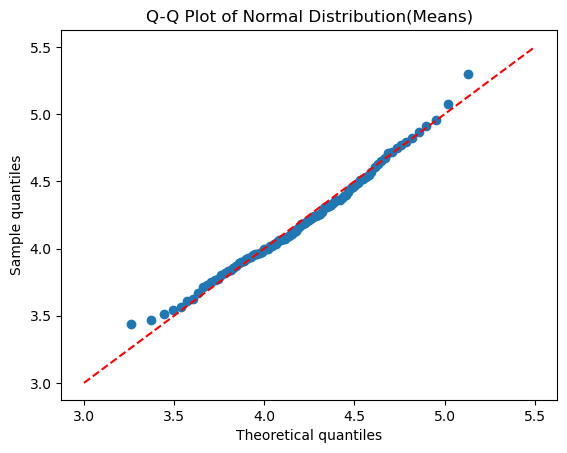
\includegraphics[width=0.3\textwidth]{qqm.png}}% 子图1的相对位置
	\subfigure[Standard Deviation]{				% 图片2
		\label{fig:sub.floorhot1}						% 子图2的标签
		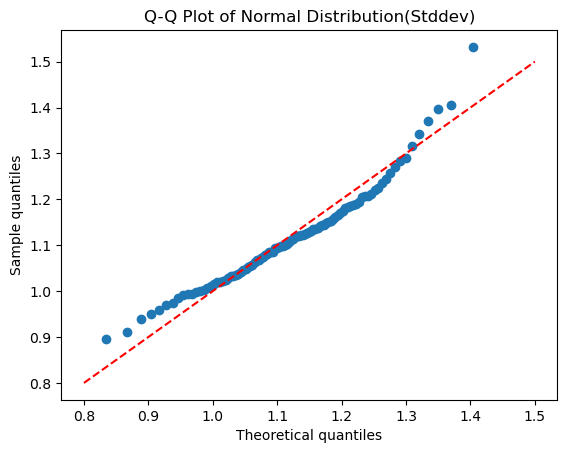
\includegraphics[width=0.3\textwidth]{qqstd.png}}% 子图2的相对位置
	\caption{the QQ plots of mean and standard deviation}		% 总图标题
	\label{}									% 总图标签
\end{figure}
% ............................End Line.....................................
% \begin{figure}[H]
% 	\centering
% 	\includegraphics[width=.6\textwidth]{.png}
% 	\caption{}
% 	\label{img}
% \end{figure}



	
	\section{Analysis on Model's Sensitivity}

	In TASK 5, a support vector machine classification model was used to classify the specified word difficulty based on 4 word attributes. To determine the effect of the 4 attributes on the final classification results, here we performed a sensitivity analysis.
	
	For each of the 4 word attributes in the dataset fluctuated from 0.1 to 0.5, respectively, and were again brought into the support vector machine classification model for classification prediction to test the accuracy between the test and prediction sets, where word frequency, MNRL, and word root fluctuations were found to fluctuate in the interval 0.1 to 0.3, and the accuracy was still high, and it can be assumed that the sensitivity of these attributes in the interval to the final classification results is small.
	
	When the fluctuation is between 0.1 and 0.4, the accuracy of the 4 attributes of the word brought back into the model is as follows:
	
	\begin{figure}[H]
		\centering
		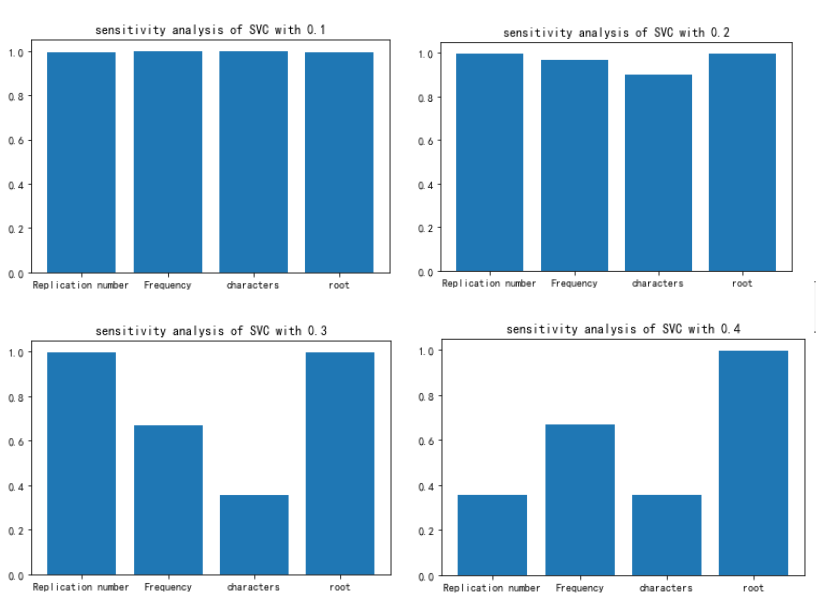
\includegraphics[width=.6\textwidth]{pic8.png}
		\caption{Sensitivity analysis graph for each word attribute in different intervals}
		\label{img}
	\end{figure}




% 以下为信件/备忘录部分,不需要可自行去掉
% 如有需要可将整个 letter 环境移动到文章开头或中间
% 请在后一个花括号内填写信件(Letter)或备忘录(Memorandum)标题
%审视艺术家和流派的进化和革命趋势
\begin{letter}{Our Letter}
	\begin{flushleft}  % 左对齐环境,无首行缩进
	Dear Editor:
	\end{flushleft}

We would like to submit the enclosed manuscript entitled “Paper Title”, which we wish to be considered for publication in “New York Times”. No conflict of interest exits in the submission of this manuscript, and manuscript is approved by all authors for publication. I would like to declare on behalf of my co-authors that the work described was original research that has not been published previously, and not under consideration for publication elsewhere, in whole or in part. All the authors listed have approved the manuscript that is enclosed.

In this problem, we used the corpus to collect the four indicators of word frequency, MNRL, lexicality, and root word to build features of words to facilitate subsequent model building.

For problem 1, the ADF test is satisfied by the difference method, and we use the ARIMA model to predict the number of people, and since the predicted value is an exact value, but to avoid absolutes, we use the confidence interval as the prediction interval. The predicted interval is [0,49485]. We targeted the correlation analysis of the four features of the words with the two indicators of the distribution of the number of response attempts using different methods of calculating the correlation coefficient. The results of the analysis found that the maximum number of repeated words significantly affects the percentage of player attempts in the difficult mode, and the larger the MNRL, the higher the percentage of players with multiple attempts and the lower the percentage with fewer attempts. The other three indicators do not correlate well with the percentage of attempts.

For problem 2, we used the data from the dataset and built a linear regression model to predict the mean as well as the standard deviation of the number of player attempts from the four indicators of the word and the date. We used the mean of the number of attempts as $\mu$ and the standard deviation of the number of attempts as $\sigma$ to establish a normal distribution as a probability model for the percentage of player attempts. Since the number of attempts here is discrete and there are only seven, we calculate the percentage of specific attempts by integration. We predicted the mean value of the number of attempts for the word eerie on March 1, 2023 to be 4.82, with a standard deviation of 1.12. Therefore, a normal distribution was created and discretized to calculate the percentage result as ("1 try":0.0015, "2 tries":0.0176, "3 tries":0.1001, "4 tries":0.2683, "5 tries":0.3406, "6 tries":0.2051, "more than 7 tries":0.0584)

For problem 3, we built a hierarchical clustering model based on four word features to file the difficulty of all words. The WSS formula was also used to measure the contribution of the 4 indicators of word attributes to the results, where the largest contribution was made by MNRL. Subsequently, a support vector machine model was built based on the specific data to analyze the word attributes of the word EERIE as difficulty.

For problem 4, we deeply mined the dataset and found some interesting characteristics, such as the mean and variance of the number of player attempts satisfy normal distribution; the more the number of all players, the smaller the percentage of difficult mode players; the number of difficult mode players grows slowly over time, etc.

We deeply appreciate your consideration of our manuscript, and we look forward to receiving comments from the reviewers. 

Thank you and best regards.
%此处引用


\hfill Yours Sincerely,

\hfill Team $\#$2307519  
\end{letter}

% \clearpage
\begin{thebibliography}{99}
	\bibitem{1} D. E. Rumelhart, G. E. Hinton, and R. J. Williams, “Learning representations by back-propagating errors,” Nature, vol. 323, no. 6088, pp. 533–536, 1986.
	\bibitem{2} T. Cover  P. Hart, "Nearest neighbor pattern classification," Journal IEEE Transactions on Information Theory archive Volume 13 Issue 1, January 1967
	\bibitem{3} 彭天奎. 正态分布偏化、离散化研究及其应用[D].重庆理工大学,2021.DOI:10.27753/d.cnki.gcqgx.2021.000013.
	\bibitem{4} 李振亮,乐昕雨.基于ARIMA模型的北京市GDP分析与预测[J].中小企业管理与科技,2023,No.694(01):153-155.
	\bibitem{5} Ying Wang, Weiwei Cheng, Chang Liu. Research on deduplication method of multiple relations based on hierarchical clustering algorithm[J]. International Journal of Information and Communication Technology,2023,22(2).
	\end{thebibliography}

\begin{appendices}
	Source Code : 
\end{appendices}
\end{document}  % 结束$
%http://www.360doc.com/content/14/0505/10/15883912_374732455.shtml
%Task5里的参考文献